% EventGPT paper (working draft)
% Compile with XeLaTeX (run twice for references): xelatex eventgpt.tex
% Numbers marked \tbd are pending runs; every other number is measured on MBD-mini.
\documentclass[12pt]{article}
\usepackage{fontspec}
\usepackage[protrusion=true]{microtype}
\usepackage{geometry}
\geometry{margin=1in}
\usepackage{graphicx}
\usepackage{amsmath}
\usepackage{booktabs}
\usepackage{siunitx}
\sisetup{table-format=1.3, table-number-alignment=center}
\usepackage[dvipsnames]{xcolor}
\usepackage[hidelinks]{hyperref}
\usepackage{url}
\usepackage{setspace}
\usepackage[font=small,labelfont=bf,skip=6pt]{caption}
\usepackage{titlesec}
\titlespacing*{\section}{0pt}{1.2em}{0.6em}
\titlespacing*{\subsection}{0pt}{1em}{0.5em}
\titlespacing*{\subsubsection}{0pt}{0.9em}{0.4em}
\usepackage{enumitem}

% --- figures: drawn in Illustrator, sources in figures/src/*.ai, included as vector PDF ---
\definecolor{capblue}{HTML}{2C6FB5}
\definecolor{capred}{HTML}{C0392B}
\definecolor{capgray}{HTML}{7F8C8D}
\definecolor{capgreen}{HTML}{2E8B57}

% --- math font: match the Latin Modern text (load last, after amsmath/fontspec) ---
\usepackage{unicode-math}
\setmathfont{latinmodern-math.otf}

% No first-line indent; one consistent line of space between paragraphs
\setlength{\parindent}{0pt}
\setlength{\parskip}{0.6em}
\setlist{leftmargin=2em, itemsep=0.25em, topsep=0.5em, partopsep=0pt}
\setlength{\abovedisplayskip}{0.5em}
\setlength{\belowdisplayskip}{0.5em}
\setlength{\abovedisplayshortskip}{0.3em}
\setlength{\belowdisplayshortskip}{0.3em}

% shorthands
\newcommand{\tbd}{\textcolor{capred}{\textbf{TBD}}}
\newcommand{\note}[1]{\textcolor{capred}{[#1]}}
\newcommand{\tok}[1]{\texttt{#1}}

\begin{document}
\onehalfspacing

\title{EventGPT: Next-Event Pretraining\\on Customer Event Histories}
\author{Denis Burakov}
\date{October 2026 (working draft)}
\maketitle

\begin{abstract}
\noindent
A model pretrained to predict a customer's next event can score questions about future events with no
labels. We pretrain EventGPT, a causal transformer, by next-token prediction on the public Multimodal
Banking Dataset (MBD-mini, 100,224 clients, 38.8 million transactions and 66.3 million geolocation pings)
and score five targets of the form ``the client makes a transaction of a given kind for the first time
next month'' from its next-event distribution alone. These zero-shot scores reach ROC-AUC 0.79 to 0.92,
against 0.84 to 0.93 for a logistic head fitted on labels, and exceed the head on two of the five
targets. Read as a frozen embedding, EventGPT reaches a mean ROC-AUC of 0.774 on MBD's four product
targets, level with a table of token counts over the same 2,048-token window (0.777), which needs no
knowledge of the schema. Gradient boosting on 114 hand-built features of the full history reaches 0.815,
and the 0.038 between the two tables decomposes into history length (0.026) and schema knowledge (0.012). The embedding at a cut
depends only on events before it, so it can be stored as a point-in-time feature. EventGPT pools each
event into one vector and decodes the next event from the history state before it; as an embedding it is
level with a flat decoder of the same size (0.774 against 0.777), from one state where the flat decoder
pools 256, and it trains 2.5 times faster.
\end{abstract}

% -------------------------------------------------------------------------------
\section{Introduction}\label{sec:intro}

A model pretrained to predict a customer's next event can be used in two ways. It can answer questions
about future events directly, from its own predictions and without labels, and it can give one
representation per customer that supervised tasks share through small heads. EventGPT is trained by
predicting each next token of a customer's event stream. This paper describes the architecture and
measures both uses on a public banking benchmark.

The usual alternative is a feature table: counts, sums and recencies computed per customer and window,
with a gradient-boosted model fitted per label. Building the table takes knowledge of the schema (which
field is the amount, which event types matter, which windows), and that work is repeated for every new
event source. Each new question then needs labels and a model of its own. When events of many kinds with
different fields are combined, as in a lender's applications, repayments and account events, there is
often no obvious table to build. A pretrained event model needs neither the table nor, for questions
about events, the labels.

We measure three things. First, how well the next-event distribution scores event targets with no labels
(Section~\ref{sec:zero-shot}). Second, how a frozen embedding compares with a flat decoder of the same
size and with aggregate tables, one built by hand and one computed mechanically from the token stream
(Section~\ref{sec:propensity}). Third, where the remaining gap to hand-built aggregates comes from
(Section~\ref{sec:gap}).

Several financial institutions describe foundation models of this kind. Nubank's nuFormer is a flat
causal decoder over customer transaction tokens \cite{nuformer}, Revolut's PRAGMA is a masked model with
separate encoders for profile state, single events and history \cite{pragma}, and Visa's TransactionGPT
encodes the aspects of each transaction before modelling across transactions \cite{transactiongpt}. None
of these releases checkpoints or evaluates on shared data, and a released checkpoint would be of little use
to another institution: its vocabulary is the issuer's own event schema, so each institution pretrains its
own backbone (Section~\ref{sec:per-institution}). EventGPT combines a per-event encoder, as in
PRAGMA and TransactionGPT, with the causal objective of nuFormer, and it was first developed on the
product histories of a consumer lender. Here we train and evaluate it only on public data so that the
results can be reproduced.

\paragraph{Contributions.}
\begin{enumerate}
\item \textbf{Zero-shot scoring of event targets} from the token decoder's distribution over the next
event, which reaches ROC-AUC within 0.05 of a supervised head on five first-occurrence targets with no
labels (Section~\ref{sec:zero-shot}).
\item \textbf{An evaluation of frozen embeddings on MBD} against a schema-free token-count table, which
is level with the embedding inside the same window, and against hand-built aggregates, with the gap to
the latter decomposed into history length, schema knowledge and amount resolution
(Sections~\ref{sec:protocol}--\ref{sec:results}).
\item \textbf{Embeddings as point-in-time features}: the conditions under which a stored embedding holds
nothing after its cut, in the architecture and in the data (Section~\ref{sec:pit}).
\item \textbf{A hierarchical decoder} that matches a flat decoder of the same size as an embedding at 2.5
times its training throughput, reading one state where the flat decoder pools 256, at the cost of a
higher token loss (Sections~\ref{sec:model} and~\ref{sec:propensity}).
\item \textbf{A tokenization of MBD} that separates static client attributes into a profile event and
thins geolocation to one event per day, which cuts the stream by 27\% with no loss of information
(Section~\ref{sec:data}).
\end{enumerate}

% -------------------------------------------------------------------------------
\section{Related work}\label{sec:related}

\paragraph{Event-sequence models in banking.} CoLES learns client embeddings by contrastive learning
on subsequences of a client's transactions \cite{coles}. TabBERT and TabGPT treat each transaction as a
row of fields, encode fields into a row embedding and model the rows with a masked or a causal
transformer \cite{tabbert}. The MBD paper evaluates these methods, aggregate features and a supervised
recurrent network on the same product-propensity task used here \cite{mbd}.

\paragraph{Industrial foundation models.} nuFormer pretrains a flat causal decoder on tokenized
transactions and fuses the embedding with a tabular network at fine-tuning time \cite{nuformer}. PRAGMA
reconstructs masked tokens with a profile-state encoder, a per-event encoder and a history encoder, and
serves credit scoring, fraud and lifetime value from one backbone \cite{pragma}. TransactionGPT applies
a three-dimensional transformer to payment-network transactions \cite{transactiongpt}. NVIDIA describes the
same recipe, tokenizer to decoder to embedding to classifier, for card transactions \cite{nvidia}.

\paragraph{Positions from time.} Rotary embeddings rotate queries and keys by an angle proportional to a
position \cite{rope}. Nothing in the rotation requires the position to be an integer, which is what lets
EventGPT feed elapsed time in its place.

% -------------------------------------------------------------------------------
\section{Model}\label{sec:model}

EventGPT has three stages (Figure~\ref{fig:arch}). An event encoder turns each event into one vector, a
history decoder models the sequence of those vectors for each client, and a token decoder predicts the
tokens of the next event. One loss, next-token cross-entropy, trains all three.

\begin{figure}[htbp]
\centering
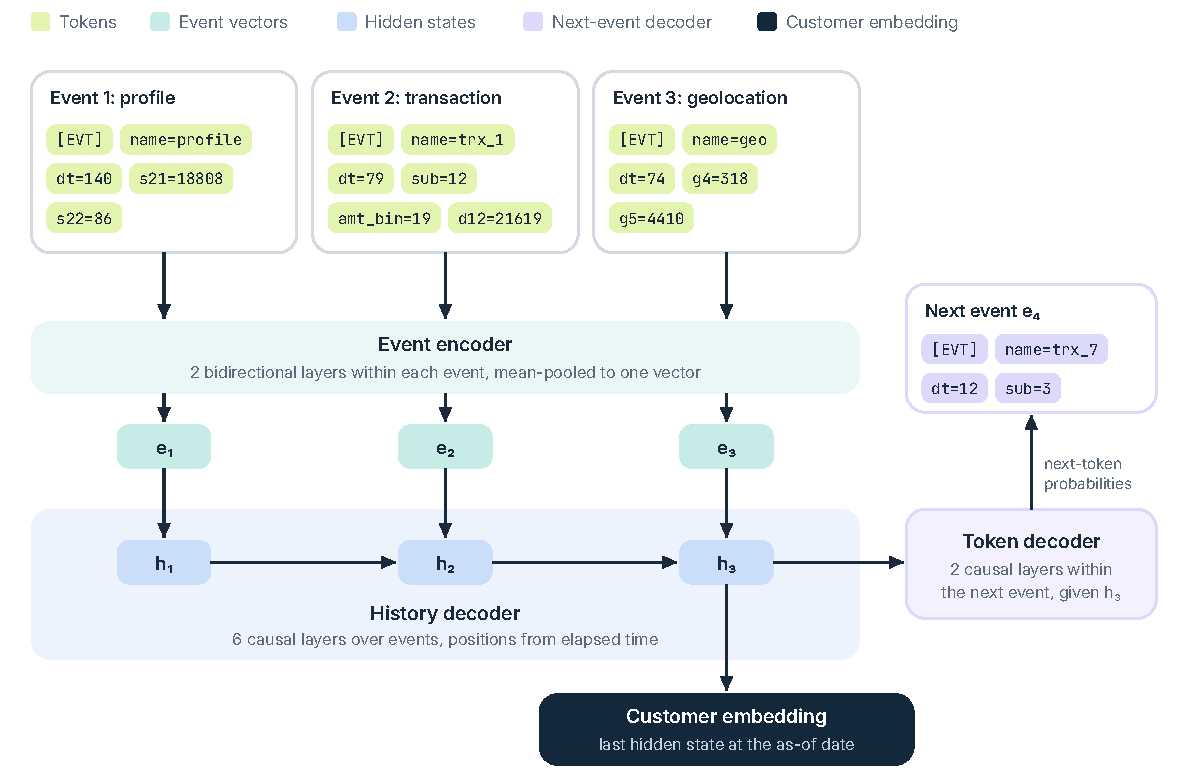
\includegraphics[width=\textwidth]{figures/hierarchy.pdf}
\caption{The three stages of EventGPT on three MBD events. Token layers read each event on its own and
mean-pool it into one vector; causal event layers with time positions model the event vectors; token
layers decode the next event given the history state of the previous one. The event layers' states are
the customer embedding; the token decoder trains them and gives the distribution of the next event.}
\label{fig:arch}
\end{figure}

\begin{figure}[htbp]
\centering
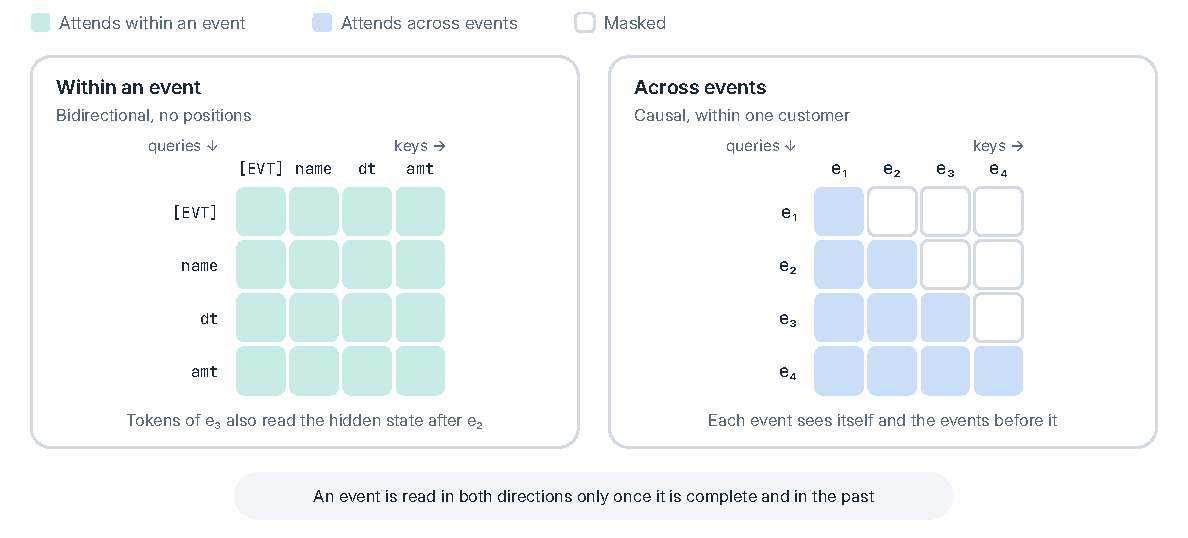
\includegraphics[width=\textwidth]{figures/attention.pdf}
\caption{Attention at the two levels. Within an event every token attends to every other; across events
attention is causal and confined to one customer. The tokens of an event reach earlier events only
through the history state of the previous event.}
\label{fig:masks}
\end{figure}

\subsection{Event encoder}

An event is a short run of tokens that starts with \tok{[EVT]}, followed by its name, its time gap and
its fields as \tok{key=value} tokens (Section~\ref{sec:data}). The fields of an event are a record, and
reading \tok{amt\_bin} before \tok{sub} states the same fact as reading them in the other order. The
encoder is therefore bidirectional within an event, has no positions inside it, and cannot attend across
an event boundary. Two layers produce token states that are mean-pooled into one vector per event.

\subsection{History decoder and time positions}\label{sec:time}

Six causal layers run over the event vectors of each client, so the history that event $i$ sees is the
vectors of events $1, \dots, i-1$, one per event, rather than their tokens. Positions are elapsed time.
With $\Delta t_i$ the seconds from the client's first event in the window to event $i$, the rotary
position is
\begin{equation}\label{eq:pos}
p_i = 64 \ln\!\left(1 + \frac{\Delta t_i}{60}\right).
\end{equation}
Rotary attention depends on the difference of two positions, which here is $64\ln$ of a ratio of
elapsed times. An hour against a minute is then as far apart as a year against a month, and two events a
year apart stay far apart even when no event lies between them (Figure~\ref{fig:time}). The elapsed times come from the
\tok{dt} tokens of the stream (each bucket mapped to its midpoint in seconds), so no timestamp enters the
model beside the tokens.

\begin{figure}[htbp]
\centering
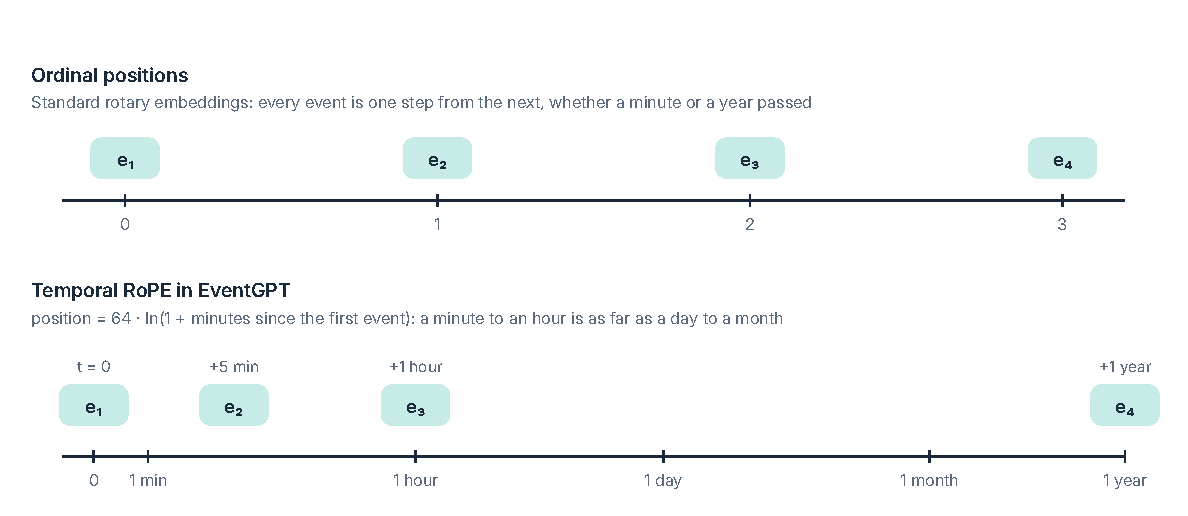
\includegraphics[width=\textwidth]{figures/time_positions.pdf}
\caption{Ordinal positions against time positions, Eq.~(\ref{eq:pos}). With ordinal positions every
event is one step from the next; with time positions the distance between two events is set by the
ratio of their elapsed times.}
\label{fig:time}
\end{figure}

\subsection{Token decoder and the training signal}

Each token of event $i$ receives its embedding, a learned position within the event and the history
state $h_{i-1}$ of the previous event; the first event in a window receives zero. Two causal layers within
the event then predict the next token through an output layer tied to the input embedding. Because the
token decoder sees $h_{i-1}$ and never the pooled vector of event $i$ itself, the bidirectional read of
an event happens only once it is complete and in the past. The event encoder has no loss of its own. Its
only gradient path runs from the pooled vector, through the history state, to the tokens of the next
event, so it keeps the fields of an event that help predict what follows.

\subsection{Packed attention within events}\label{sec:packed}

The event encoder and the token decoder never attend across an event boundary, yet a dense mask over a
window of $t$ tokens costs memory in proportion to $t^2$. We instead lay each event out as one row of at
most $L$ slots, with $L$ the longest event in the window (ten tokens on MBD), and attend within rows, so
both stages cost in proportion to the number of events times $L^2$. On real windows the packed and the
dense computations agree to within $1.2 \times 10^{-6}$ on every event. This is what makes histories of
8,192 tokens and more affordable (Section~\ref{sec:context}).

\subsection{Customer embedding}\label{sec:embedding}

The embedding of a customer at a cut is read from the history decoder's states for the events before the
cut, in one of three ways: the state after the last event (\emph{last}), the mean over events
(\emph{mean}), or a mean weighted by $\exp(-a/32)$ for an event $a$ events before the last
(\emph{recency}). One forward pass gives all three. Each history ends in a \emph{now} event,
\tok{[EVT] dt=<gap>}, whose gap runs from the last event to the cut, so the readout sits at the cut time and
two customers with the same events but different silences before the cut get different embeddings.

\section{Embeddings as point-in-time features}\label{sec:pit}

The embedding is what the pretraining is for. Computed once per customer and cut, it serves every
downstream task through a small head fitted on it, and the backbone is neither retrained nor fine-tuned
per task. In this paper one set of embeddings serves ten labels (four product targets, five event
targets and churn, Section~\ref{sec:protocol}), each through a logistic regression. A new task then costs
a head on stored vectors rather than a new model on raw events, which is the arrangement Revolut and
Nubank describe for their backbones \cite{pragma, nuformer}.

That reuse is safe only if the embedding at a cut is a function of events before the cut alone. An
embedding that has seen the future inflates the offline results of every task built on it, and because
every head inherits the embedding, the error is not confined to one model. EventGPT
guarantees the property at two levels.

\paragraph{In the architecture.} The history decoder is causal, so the state after event $i$ depends on
events $1, \dots, i$ only. The bidirectional read of the event encoder stays within one event, and the
token decoder reaches earlier events only through $h_{i-1}$, the state of the previous event; no token
of event $i$ has a path to the encoded vector of event $i$ itself. The embedding read after the last event
before a cut is therefore the same whether or not later events exist in the stream. The probe also builds
each input to end at its cut, so later events are never present in it.

\paragraph{In the data.} Point-in-time correctness also depends on how events are built, and each step of
Section~\ref{sec:data} is placed to keep it.
\begin{itemize}
\item The history for a cut is every event strictly before the first day of the month, in the bank's own
time zone.
\item A daily geolocation event is stamped at the day's last ping, so a summary of the day never appears
before the pings it summarizes.
\item The profile event carries fields that never change within a client and is stamped at the client's
first event, so it enters a history only when some event does.
\item The vocabulary and the amount-bin edges are fitted on the pretraining folds only, and the test fold
is never seen in pretraining.
\end{itemize}

Because the history prefix itself fixes the as-of time, an embedding can be stored in a feature store
like any other timestamped feature: keyed by customer, stamped with its cut rather than with the time it
was computed, and joined to labels by the store's point-in-time join, which then returns for each label
the latest embedding before it. The join chooses which snapshot a label sees; the prefix guarantees that
the snapshot itself holds nothing after its cut. Embeddings from different checkpoints are not comparable, so each backbone
version needs its own feature set, and a head is valid only on the version it was fitted on. What the guarantee does not cover is the population: pretraining reads the full
2021--2022 histories of the pretraining clients, so the backbone has seen the period in which the test
clients' labels fall, although never those clients (Section~\ref{sec:limits}).

% -------------------------------------------------------------------------------
\section{Data}\label{sec:data}

\subsection{MBD-mini}

MBD is a dataset of bank clients released for research on event sequences, with transactions,
geolocation pings and support dialogues per client, and monthly labels for the purchase of four products
\cite{mbd}. MBD-mini, a 10\% client sample of it, is published under CC BY 4.0 \cite{mbdmini}. Table~\ref{tab:mbd}
gives its size. All fields are anonymized integer codes, amounts are rescaled, and timestamps are in UTC
with the bank's day starting at 21:00 UTC (Moscow time). Clients are split into five folds of equal size.

\begin{table}[htbp]
\centering
\caption{MBD-mini sources. Events per client are the 50th, 90th and 99th percentiles.}
\label{tab:mbd}
\begin{tabular}{lrrlr}
\toprule
source & events & clients & span & per client (p50 / p90 / p99) \\
\midrule
transactions & 38.8M & 98,721 & Jan 2021 -- Dec 2022 & 170 / 1,007 / 2,243 \\
geolocation pings & 66.3M & 72,573 & Dec 2021 -- Dec 2022 & 507 / 2,293 / 5,580 \\
dialogues & 0.22M & 46,320 & Feb 2021 -- Dec 2022 & 3 / 10 / 27 \\
\bottomrule
\end{tabular}
\end{table}

\subsection{Events and tokens}

Each client's stream starts with \tok{[USR]} and a profile event, then interleaves transactions and
geolocation in time order:
\begin{center}
\small
\begin{tabular}{ll}
profile & \tok{[EVT] name=profile dt=140 s21 s22 s31 s32} \\
transaction & \tok{[EVT] name=trx\_<type> dt=<b> sub=<subtype> amt\_bin=<b> [cur] s11 s12 d11 d12} \\
geolocation & \tok{[EVT] name=geo dt=<b> g4=<cell> g5=<cell>} \\
\end{tabular}
\end{center}

\paragraph{Profile event.} The four fields \tok{src\_type21}, \tok{src\_type22}, \tok{src\_type31} and
\tok{src\_type32} never change within a client: on fold 1 they change on 0.0\% of consecutive
transactions, against 13--15\% for \tok{src\_type11} and \tok{src\_type12} and 55--63\% for the
destination fields and the event type. They are attributes of the client's account. Repeated on every transaction they took 4 of 13 tokens, so we state them once, in a profile
event at the client's first event time. Transactions fall to 9 tokens and the pretraining stream from
454 million to 332 million tokens. The profile event also gives the model what PRAGMA's profile-state
encoder provides \cite{pragma}, a representation of static attributes learned jointly with the events.

\paragraph{Geolocation.} Raw pings outnumber transactions 1.7 to 1 and would crowd them out of a
window. We keep one geolocation event per client per Moscow day, carrying the day's most frequent
\tok{geohash\_5} cell and the \tok{geohash\_4} cell that contains it, stamped at the day's last ping so
that the event never runs ahead of what it summarizes. This keeps 14.7 million events. The geohash codes
are anonymized, so no spatial adjacency can be computed, but every \tok{geohash\_5} cell lies in exactly
one \tok{geohash\_4} cell, and the shared \tok{g4} token lets cells in the same area share information.

\paragraph{Time and amounts.} The gap since the client's previous event becomes a token
\tok{dt=}$\lfloor 8 \ln(1 + \Delta s/8) \rfloor$, capped at 140, so 141 buckets span seconds to
decades. Amounts become one of 21 bins with quantile edges fitted on the pretraining folds.

\paragraph{Vocabulary.} Values seen in the pretraining folds become tokens, and values of the two
counterparty-like fields seen fewer than 1,000 times and geohash cells seen fewer than 100
(\tok{g4}) or 300 (\tok{g5}) times fall into an \tok{other} token per key. The vocabulary has 12,828
tokens, and no token of the held-out fold is unknown. Dialogue embeddings are left out of this version.

The stream holds 53.4 million events in all, about 8 tokens per event. Folds 1--4 give the pretraining
stream, with 2\% of their clients held out for validation loss: 332 million training tokens and 6.8
million validation tokens. Fold 0 is never seen in pretraining or vocabulary fitting.

% -------------------------------------------------------------------------------
\section{Evaluation protocol}\label{sec:protocol}

\subsection{Cuts and labels}

A row is a client and a month from February 2022 to January 2023, 12 per client. Following MBD, the
history for a month is every event strictly before the first day of that month \cite{mbd}, here in
Moscow time. Two kinds of label share these rows.

\paragraph{Official targets.} \tok{target\_1} to \tok{target\_4} indicate that the client takes product
$k$ during the month. They are rare: on the test fold, \tok{target\_1} has 1,072 positives in 243,936
rows (0.44\%), \tok{target\_2} 132 (0.05\%), \tok{target\_3} 934 (0.38\%) and \tok{target\_4} 634
(0.26\%). Of these rows, 1,332 belong to 111 clients with no transactions or geolocation, who have no stream; both the
probe and the baseline drop them, leaving 242,604 scored rows. No single event type marks a purchase: the event type most often seen for the first time in
the month of a purchase covers at most 10\% of its positives.

\paragraph{Event targets.} Purchases do leave traces in the stream. Among \tok{target\_2} positives, the
transaction kinds (type, subtype) 48/31, 23/49, 26/28 and 48/10 appear for the first time in the
client's history 56 to 262 times more often than among negatives, and 50/19 does so 27 times more often
among \tok{target\_3} positives. We define an event target for each of these kinds (the kind appears in
the client's history for the first time during the month) and a \emph{churn} target (no transaction
during the month from a client with at least one before the cut). These are read from the stream, as the
targets of a deployed propensity model usually are.

\subsection{Heads and metrics}

Embeddings are frozen. For each label we fit a logistic regression on standardized embeddings
($C = 0.1$) on rows from folds 1--4 and score every row of fold 0. Positives are rare, so the training
rows are every row positive for any label plus 60,000 rows sampled uniformly from the rest, reweighted
to their share. We report ROC-AUC and PR-AUC (average precision). PR-AUC matters here because a ranking
can reach a high ROC-AUC while its top is still mostly negatives; a random ranking has a PR-AUC equal to
the prevalence, which the tables give beside it.

\subsection{Zero-shot event targets}\label{sec:zs-protocol}

An event target, the kind $(X, Y)$ appearing in a client's history for the first time during the month,
can be scored by the pretrained model with no head and no labels. After the history at a cut we append
the start of a next event, \tok{[EVT] name=trx\_X dt=<g>}, where $g$ is the bucketed gap from the last
event to the cut. The token decoder gives $P(\tok{name=trx\_X})$ at \tok{[EVT]} and
$P(\tok{sub=Y} \mid \tok{name=trx\_X}, \tok{dt=g})$ at the \tok{dt} token, and the score is their product,
the probability that the next event is of kind $(X, Y)$. A client who already had the kind before the cut
cannot be positive under the label's definition, so that client's score is set to zero. This rule uses
no labels, and we apply it to the supervised scores as well when comparing the two. The history stages run
once per row and the token decoder once per type $X$.

Zero-shot scoring is evaluated on every test row positive for one of the five event targets and on
20,000 rows sampled uniformly from the test fold. Each target's ROC-AUC uses its own positives and the
uniform sample, so the positives of the other targets do not enter as negatives, and uniform sampling
of negatives leaves ROC-AUC unbiased. The supervised comparison is the logistic head on the last
readout, scored on the same rows.

\subsection{Baselines}

\paragraph{Aggregate features.} On the same rows we compute 114 features from events before the cut:
transaction counts and amount sum, mean and maximum, count and amount per event type for the 15 most
frequent types, geolocation pings and active days, each over all history, the last month and the last
three months, together with days since the first and last transaction and the four profile fields as
categorical features. CatBoost \cite{catboost} (depth 6, learning rate 0.05, at most 2,000 trees with
early stopping on 10\% of training clients) is fitted per label on the same training rows. These
features need the schema: which table holds transactions, which field is the amount and which event
types are frequent.

\paragraph{Token counts.} A table that needs no knowledge of the schema: for each of the 200 most frequent
tokens of the stream (any \tok{key=value}, amount bin or time bucket, 90.9\% of all non-special tokens),
its count over all history, the last 91 days and the last 30 days, with the number of events in each
window and the days since the first and the last event, 605 features in all. It is computed either over
the full history or over the same 2,048-token window that EventGPT reads, and fitted with the same
CatBoost settings. Any tokenized event stream with timestamps yields this table, so it is the
alternative an institution has when no one has written features for its events.

\paragraph{Flat decoder.} A GPT-style decoder of width 384 with ten layers and learned positions over
the same token stream, 23.5 million parameters against EventGPT's 22.9 million, trained identically. It
has no event states, so its readouts run over tokens: the last token, the mean over tokens and a recency
weight over about 256 tokens, as many as 32 events hold.

\paragraph{Published results.} The MBD paper reports mean ROC-AUC on full MBD, a population ten times
larger with its own five-fold split (Table~\ref{tab:published}). These numbers give context only:
MBD-mini is a different sample, and the comparison on full MBD is planned
(Section~\ref{sec:limits}).

\begin{table}[htbp]
\centering
\caption{Mean ROC-AUC over the four product targets on full MBD, as reported by \cite{mbd} (late fusion
for the two-source column).}
\label{tab:published}
\begin{tabular}{lcc}
\toprule
method & transactions & transactions + geo \\
\midrule
aggregation & 0.783 & \\
CoLES & 0.773 & 0.775 \\
TabBERT & 0.762 & 0.764 \\
TabGPT & 0.802 & 0.800 \\
supervised RNN & 0.819 & 0.819 \\
\bottomrule
\end{tabular}
\end{table}

\subsection{Training}

EventGPT has width 384, 12 heads of width 32, two event-encoder layers, six history layers and two
token-decoder layers: 22.9 million parameters, of which 4.9 million are the tied token embedding. It is
trained with AdamW (learning rate $6 \times 10^{-4}$, $\beta = (0.9, 0.95)$, weight decay 0.1), linear
warmup for 200 steps and cosine decay to 10\% of the peak, on windows of 2,048 tokens drawn at uniform
offsets from the packed stream, 16 windows (32,768 tokens) per step, for 20,000 steps, about two passes
over the data. Windows start mid-event and mid-client; \tok{[USR]} tokens bound the attention of each
client. On one NVIDIA L4 in bfloat16 a run of 655 million tokens takes 1.5 hours (about 118,000 tokens
per second), against 3.9 hours (about 47,000) for the flat decoder. Every model is trained with two
seeds, 42 and 43, and model results are the mean of the two unless stated.

% -------------------------------------------------------------------------------
\section{Results}\label{sec:results}

\subsection{Event targets without labels}\label{sec:zero-shot}

Scored from the next-event distribution alone, the five event targets reach ROC-AUC 0.79 to 0.92
(Table~\ref{tab:zero-shot}). A logistic head fitted on labels reaches 0.84 to 0.93 on the same rows.
The zero-shot score is higher on 48/31 and 50/19, within 0.012 on 23/49, and lower by 0.046 to 0.048 on
26/28 and 48/10. The two seeds differ by at most 0.014, on 48/31, which has 59 positives. On 23/49 the
zero-shot score also exceeds gradient boosting on the hand-built aggregates, which is fitted on labels.

\begin{table}[htbp]
\centering
\caption{ROC-AUC on the five event targets. Zero-shot scores use no labels; both EventGPT columns set
the score of clients who already had the kind to zero (Section~\ref{sec:zs-protocol}). The supervised
head is the logistic head on the seed-42 embedding, on the same rows. The aggregates column is the
full test fold, so it is comparable in expectation but not row for row.}
\label{tab:zero-shot}
\begin{tabular}{lrcccc}
\toprule
 & & \multicolumn{2}{c}{EventGPT zero-shot} & EventGPT & aggregates \\
target & positives & seed 42 & seed 43 & supervised head & (CatBoost) \\
\midrule
first 48/31 & 59 & 0.916 & 0.902 & 0.891 & 0.913 \\
first 23/49 & 195 & 0.918 & 0.918 & 0.930 & 0.909 \\
first 26/28 & 252 & 0.829 & 0.827 & 0.875 & 0.869 \\
first 48/10 & 290 & 0.791 & 0.784 & 0.836 & 0.842 \\
first 50/19 & 770 & 0.906 & 0.904 & 0.896 & 0.936 \\
\bottomrule
\end{tabular}
\end{table}

The rule for earlier occurrences matters most where the kind is common. Without it, 50/19 falls from
0.906 to 0.722 (seed 42), because the model predicts the kind for clients who already make it every
month; the rule changes 48/31, a rare kind, by 0.001. The score is the probability of the kind as the
\emph{next} event, while the label covers the whole month. Sampling a month of events from the model
and testing for the kind would match the label's horizon; we have not run it.

\subsection{Frozen embeddings with a supervised head}\label{sec:propensity}

Table~\ref{tab:main} gives every label for the embeddings and the baselines.

\begin{table}[htbp]
\centering
\small
\setlength{\tabcolsep}{4pt}
\caption{ROC-AUC on the test fold. Model columns are the mean of two seeds, with a logistic head on the
frozen readout. Token counts and aggregates are fitted with CatBoost. PR-AUC for the official targets
is in Table~\ref{tab:main-pr}.}
\label{tab:main}
\begin{tabular}{lcccccc}
\toprule
 & aggregates & \multicolumn{2}{c}{token counts} & \multicolumn{2}{c}{flat decoder} & EventGPT \\
target & full history & full history & 2,048 tokens & last & recency & last \\
\midrule
\tok{target\_1} & 0.787 & 0.781 & 0.757 & 0.692 & 0.738 & 0.740 \\
\tok{target\_2} & 0.835 & 0.849 & 0.792 & 0.725 & 0.823 & 0.829 \\
\tok{target\_3} & 0.818 & 0.809 & 0.788 & 0.729 & 0.783 & 0.776 \\
\tok{target\_4} & 0.819 & 0.774 & 0.770 & 0.709 & 0.765 & 0.753 \\
mean & 0.815 & 0.803 & 0.777 & 0.714 & 0.777 & 0.774 \\
\midrule
first 48/31 & 0.913 & 0.905 & 0.913 & 0.794 & 0.909 & 0.889 \\
first 23/49 & 0.909 & 0.905 & 0.915 & 0.796 & 0.918 & 0.918 \\
first 26/28 & 0.869 & 0.879 & 0.874 & 0.745 & 0.844 & 0.860 \\
first 48/10 & 0.842 & 0.857 & 0.846 & 0.715 & 0.793 & 0.804 \\
first 50/19 & 0.936 & 0.935 & 0.922 & 0.769 & 0.856 & 0.837 \\
churn & 0.961 & 0.960 & 0.958 & 0.776 & 0.804 & 0.830 \\
\bottomrule
\end{tabular}
\end{table}

\begin{table}[htbp]
\centering
\small
\setlength{\tabcolsep}{4pt}
\caption{PR-AUC on the official targets, with the prevalence a random ranking would reach.}
\label{tab:main-pr}
\begin{tabular}{lccccccc}
\toprule
 & & aggregates & \multicolumn{2}{c}{token counts} & \multicolumn{2}{c}{flat decoder} & EventGPT \\
target & prevalence & full history & full & 2,048 tokens & last & recency & last \\
\midrule
\tok{target\_1} & 0.0044 & 0.021 & 0.020 & 0.016 & 0.011 & 0.012 & 0.013 \\
\tok{target\_2} & 0.0005 & 0.012 & 0.009 & 0.016 & 0.006 & 0.008 & 0.010 \\
\tok{target\_3} & 0.0038 & 0.021 & 0.020 & 0.015 & 0.011 & 0.015 & 0.012 \\
\tok{target\_4} & 0.0026 & 0.017 & 0.013 & 0.010 & 0.007 & 0.011 & 0.010 \\
\bottomrule
\end{tabular}
\end{table}

\paragraph{Hierarchy against the flat decoder.} As embeddings the two are level. EventGPT's state after
the last event reaches a mean of 0.774 on the official targets, and the flat decoder reaches 0.777 when
its recency readout pools about 256 token states (0.786 and 0.768 on the two seeds, against 0.7741 and
0.7745 for EventGPT). Read at one state, the flat decoder's last token reaches 0.714 and is lower than
EventGPT on all ten labels in both seeds. Of the other labels, EventGPT is higher on churn (0.830 against
0.804) and on two event targets, the flat decoder on two, and 23/49 is tied. The trade is in training:
EventGPT runs at 2.5 times the throughput, and its token loss is higher (validation loss 1.020 against
0.944 and 0.947), because the token decoder sees the past only through the history state of the previous
event. The fields that repeat from recent events show it most: the flat decoder predicts the next
\tok{geohash\_5} cell with top-1 accuracy 0.68, EventGPT with 0.57, while for the event name, which
depends on the history as a whole, they are level (0.574 and 0.58). Next-token loss therefore does not rank the two as embeddings.

\paragraph{Against aggregate tables.} With the same 2,048-token window, EventGPT's last state (0.774)
and the token-count table (0.777) are level on the official targets. CatBoost fitted on EventGPT's last
and mean states reaches 0.786 (seed 42). Over the full history, token counts reach 0.803 and the
hand-built aggregates 0.815. On churn the token-count table reaches 0.958 even within the window, against
0.830 for EventGPT. The table keeps the profile event's timestamp in every window and so knows how long a
client has banked, while EventGPT sees only gaps between events.

\subsection{Where the gap to aggregates comes from}\label{sec:gap}

Three measurements locate the gap of 0.041 on the official targets between EventGPT (0.774) and the
hand-built aggregates (0.815).

\paragraph{History length.} Token counts lose 0.026 when they are restricted to EventGPT's window (0.803
against 0.777), and within the window they and EventGPT are level. A longer window is the change most
likely to close the gap (Section~\ref{sec:context}).

\paragraph{Schema knowledge.} Hand-built features add 0.012 over full-history token counts (0.815 against
0.803). This is the part that needs someone who knows which field is the amount and which event types
matter.

\paragraph{Amount resolution.} EventGPT sees amounts as one of 21 quantile bins. Replacing each amount in
the hand-built table by the mean of its bin gives 0.810 with 21 bins and 0.815 with 256 bins, against
0.815 with exact amounts. Most of the 0.005 lost with 21 bins is on \tok{target\_2}, whose 132 test
positives make it the noisiest target; the other three official targets lose 0.001 to 0.003.

Adding 32 principal components of the EventGPT embedding to the hand-built table leaves the mean at
0.815 (seed 42, embedding read without the now event). Where good aggregates exist, the embedding adds
nothing measurable on these targets.

\subsection{Ablations}

Each ablation changes one element (Table~\ref{tab:ablations}), measured with two seeds except where
marked.

\begin{table}[htbp]
\centering
\caption{Mean ROC-AUC over the official targets, logistic head, mean of two seeds.}
\label{tab:ablations}
\begin{tabular}{llc}
\toprule
element & variant & mean ROC-AUC \\
\midrule
architecture & hierarchy (EventGPT), last state & 0.774 \\
 & flat decoder, last token & 0.714 \\
 & flat decoder, recency over tokens & 0.777 \\
sources & transactions + geolocation & 0.774 \\
 & transactions only & \tbd \\
readout & last / mean / recency & 0.774 / 0.755 / 0.765 \\
\bottomrule
\end{tabular}
\end{table}

\subsection{Length of history}\label{sec:context}

A flat decoder's history is bounded by tokens and its attention cost grows with their square. The
history decoder of EventGPT attends over events, and with packed attention its token stages grow
linearly with the window. MBD histories are long (the 90th percentile client has about 1,000
transactions and 300 days of geolocation), while a 2,048-token window holds about 250 events. Token
counts lose 0.026 on the official targets when cut to this window (Section~\ref{sec:gap}), which bounds
what a longer window could give EventGPT. A window also hides how long a client has banked; a tenure
token in the profile event would restore it for churn.
\note{Figure: mean ROC-AUC against window length (2,048, 4,096, 8,192 tokens) for EventGPT and the flat
decoder, with training throughput and memory per window.}

% -------------------------------------------------------------------------------
\section{Pretraining per institution}\label{sec:per-institution}

An event model is pretrained by each institution on its own events, and what transfers between
institutions is the method: the architecture, the rules that turn an event into tokens, and the training
procedure. The weights do not transfer the way a language model's do. A language model reads text through
a vocabulary that any user shares, so one pretrained checkpoint serves any text written in its languages.
An event model's vocabulary is the issuer's event schema. Its tokens name the event types, field codes and
categories of one bank's systems, and its amount bins are quantiles of that bank's amounts.

MBD shows each layer of this. Every field is an integer code assigned by the bank, so \tok{name=trx\_1}
or \tok{s21=18808} means nothing outside it. The 12,828 tokens and the 21 amount-bin edges were fitted on
the pretraining folds of this one population, and a token id has its meaning only together with the
vocabulary file it was fitted with. Even within one institution, fitting the vocabulary again assigns ids
anew, so we store a fingerprint of the vocabulary with every checkpoint and refuse to score a checkpoint
against a vocabulary it was not trained on. The time-gap tokens are the exception, since
$\lfloor 8\ln(1 + \Delta s/8) \rfloor$ means the same at every bank.

Serving such a model therefore starts with pretraining on the institution's own history, and the
comparisons in this paper are between methods trained on the same data. Privacy and competition keep the
checkpoints of the industrial models in Section~\ref{sec:related} private in any case; the vocabulary means
that another institution could not use one without its issuer's schema.

\section{Limitations}\label{sec:limits}

The results are on MBD-mini, for which no published numbers exist, so the comparison with the MBD paper's
methods (Table~\ref{tab:published}) waits for a run on full MBD. The embeddings are evaluated frozen with
a linear head; the supervised recurrent network of \cite{mbd} is trained on the labels end to end, and a
fair answer to it is a fine-tuned or fused model. The events of MBD are mostly
transactions with one field layout, which gives the event encoder less to do than histories that mix
applications, repayments and other kinds of event with different fields. Zero-shot scoring covers only targets that are events in
the stream: MBD's product targets are external labels and need a head. It scores the next event rather
than the month, and its comparison with the supervised head is on a sample of the test fold. All results
are on one test fold. The geolocation stream starts a
year after the transactions, so early cuts carry little of it. Dialogue embeddings are not used.
The split is by client, as in MBD: pretraining reads the pretraining clients' events from 2021 to 2022,
including the months in which the test clients' labels fall. Each test history is cut before its label
month, but the backbone has learned population patterns from that period. An out-of-time evaluation would
pretrain on events before February 2022 only.

% -------------------------------------------------------------------------------
\section{Code and data availability}\label{app:code}

The code (tokenization, model, training, probe and baseline) is at \note{repository URL}. MBD-mini is
available on the Hugging Face Hub as \tok{ai-lab/MBD-mini} under CC BY 4.0 \cite{mbdmini}.

\begin{thebibliography}{99}

\bibitem{coles} Babaev, D., Ovsov, N., Kireev, I., Ivanova, M., Gusev, G., Nazarov, I., and Tuzhilin, A.
(2022). CoLES: Contrastive learning for event sequences with self-supervision. In \emph{Proceedings of the
2022 International Conference on Management of Data (SIGMOD)}. \note{verify author list and venue}

\bibitem{catboost} Prokhorenkova, L., Gusev, G., Vorobev, A., Dorogush, A.~V., and Gulin, A. (2018).
CatBoost: unbiased boosting with categorical features. In \emph{Advances in Neural Information
Processing Systems 31}.

\bibitem{mbd} Multimodal Banking Dataset: Understanding Client Needs through Event Sequences (2024).
arXiv:2409.17587. \note{add authors}

\bibitem{mbdmini} MBD-mini. Hugging Face dataset \tok{ai-lab/MBD-mini}, CC BY 4.0.
\url{https://huggingface.co/datasets/ai-lab/MBD-mini}.

\bibitem{nuformer} nuFormer (Nubank) (2025). arXiv:2507.23267. \note{add authors and title}

\bibitem{nvidia} NVIDIA. Build your own transaction foundation model for financial intelligence.
\url{https://developer.nvidia.com/blog/build-your-own-transaction-foundation-model-for-financial-intelligence/}.

\bibitem{pragma} PRAGMA (Revolut) (2026). arXiv:2604.08649. \note{add authors and title}

\bibitem{rope} Su, J., Lu, Y., Pan, S., Murtadha, A., Wen, B., and Liu, Y. (2021). RoFormer: Enhanced
transformer with rotary position embedding. arXiv:2104.09864.

\bibitem{tabbert} Padhi, I., Schiff, Y., Melnyk, I., Rigotti, M., Mroueh, Y., Dognin, P., Ross, J., Nair,
R., and Altman, E. (2021). Tabular transformers for modeling multivariate time series. In \emph{ICASSP
2021}. \note{verify}

\bibitem{transactiongpt} TransactionGPT (Visa Research) (2025). arXiv:2511.08939. \note{add authors and
title}

\end{thebibliography}

\end{document}
